\documentclass{article}
\usepackage[utf8]{inputenc}
\usepackage[english]{babel}
\usepackage{graphicx}
\usepackage{float}
\usepackage{upgreek}
\usepackage{pdfpages}
\usepackage{url}
\usepackage{subcaption}
\setlength{\parskip}{1em}
\usepackage{amsmath}
\usepackage{minted}

\usepackage[hybrid]{markdown}

\usepackage{cite}

\usepackage[a4paper, total={6in, 8in}]{geometry}
\geometry{legalpaper, portrait, margin=1in}

\title{2EL1730 - Kaggle Challenge}
\author{Alicia Rakotonirainy, Matthias Lesage, Mustapha Ajeghrir, Tony Wu \\ \\ Team GroundTruth - 5th}
\date{February 2020}

\begin{document}

\maketitle

\clearpage

\section{Feature engineering}
\subsection{Motivation and intuition behind each feature}

\begin{markdown}
- Date formatting

The strings were in an unusual format, thus it was necessary to modify before giving it to the `pd.to_datetime` function. To do this, we have used Regular Expression (also called *Regex*) with capturing groups to correctly format the string. The following Regex was used:

```python
pattern = r'(\d{1,2}.*\d{2}:\d{2}:\d{2}) ([+-]\d{2}\d{2})'
```

What this code does is to retrieve what's inside the parenthesis (capturing groups) given some conditions on the characters before and after them. We thought that the "date" feature contained a lot of informations that we should separate : for instance, there may be more of a certain type of mail during the weekends, no matter the month we have. We wanted to give the model access to the knowledge of temporality, because otherwise it wouldn't have been able to deduce ir from the string alone. We therefore created 6 separated columns : the day of the week, the hour, the month, the year, the timezone and the daymonth (concatenation of day and month). The timezone should approximately reflect a geographical information.

- Non linear relationships

We wanted to take non linear relations between features into account by creating new columns with products or divisions of different pairs of existing features : `chars_in_subject/body`, `chars_in_subject/body`, `images/body`, `salutaions&designation`, `sub/body`, `urls/body`, `images/body`, `salutations&designation`. It seems relevant for prediction : for instance, `images/body` gives the text density of the mail and we can easily think that a mail with a high ratio is more likely to be related to promotions or spam.

- TLD preprocessing

We did a OneHotEncoding for the tlds. But we transformed the values first. We have split the name value of a tld at each point (`"."`) ; for instance, `google.com` would count for 1 in the column `google`, 1 in the column `com`, and 0 elsewhere. We did so because we thought that a tld `google.fr` or `google.com` gives more or less the same information. We also standardized all the values to lower letters. Moreover, we decided to have a threshold and to take into account only the categories that appear more than this threshold ; the others fall in the category `other`. We also added a column that gives the "depth" of the tld, that is to say the number of points that it contains. 

- Org preprocessing

We applied a OneHotEncoding, using also a threshold in order to take into account only the values that appear at least a given number of times ; by doing so we reduce the curse of dimensionality. We also standardized all the values to lower letters. 

- Mailtype preprocessing

We first standardized all the values to lower letters. Then we used OneHotEncoding to represent this features, but we separated the two terms of each value : for instance `multipart/mixed` would be encoded by a 1 in the column `multipart`, a 1 in the column `mixed` and zero elsewhere. 


- Images and urls preprocessing

Since there are extremely high numerical values for a few rows, we added a threshold in order to have bounded values ; if the value exceed a given value, we replace it by the value of the threshold.

All the categorical features are cleaned from the missing values using a constant strategy : we replaced them by the str `"None"` ; for the binary columns, we replaced the NaNs with the value 0. The missing data from the numerical features were replaced by the mean of the column.

- Mean Encoding / Target Encoding (Rejected):
The idea is to replace the given categorical column by a column containing the mean target value per unique original value. Using this method, we could avoid to have much more columns thus to get rid of the *Curse of dimensionality*. However, this encoding method didn't provide great results and was therefore put aside.

\end{markdown}

\subsection{Predictive performance and feature selection}

\begin{table}[h!]
\begin{center}
 \begin{tabular}{|c | c | c | c | c | c |} 
 \hline
  669 & 670 & 668 & 667 & 664 & 28 \\ 
  \hline
  chars in subject/body & urls/body & chars in body & chars in subject & urls & minute \\
  \hline
\end{tabular}
\end{center}
\caption{Names of the principal explaining features}
\end{table}



\begin{figure}[h]
\centering
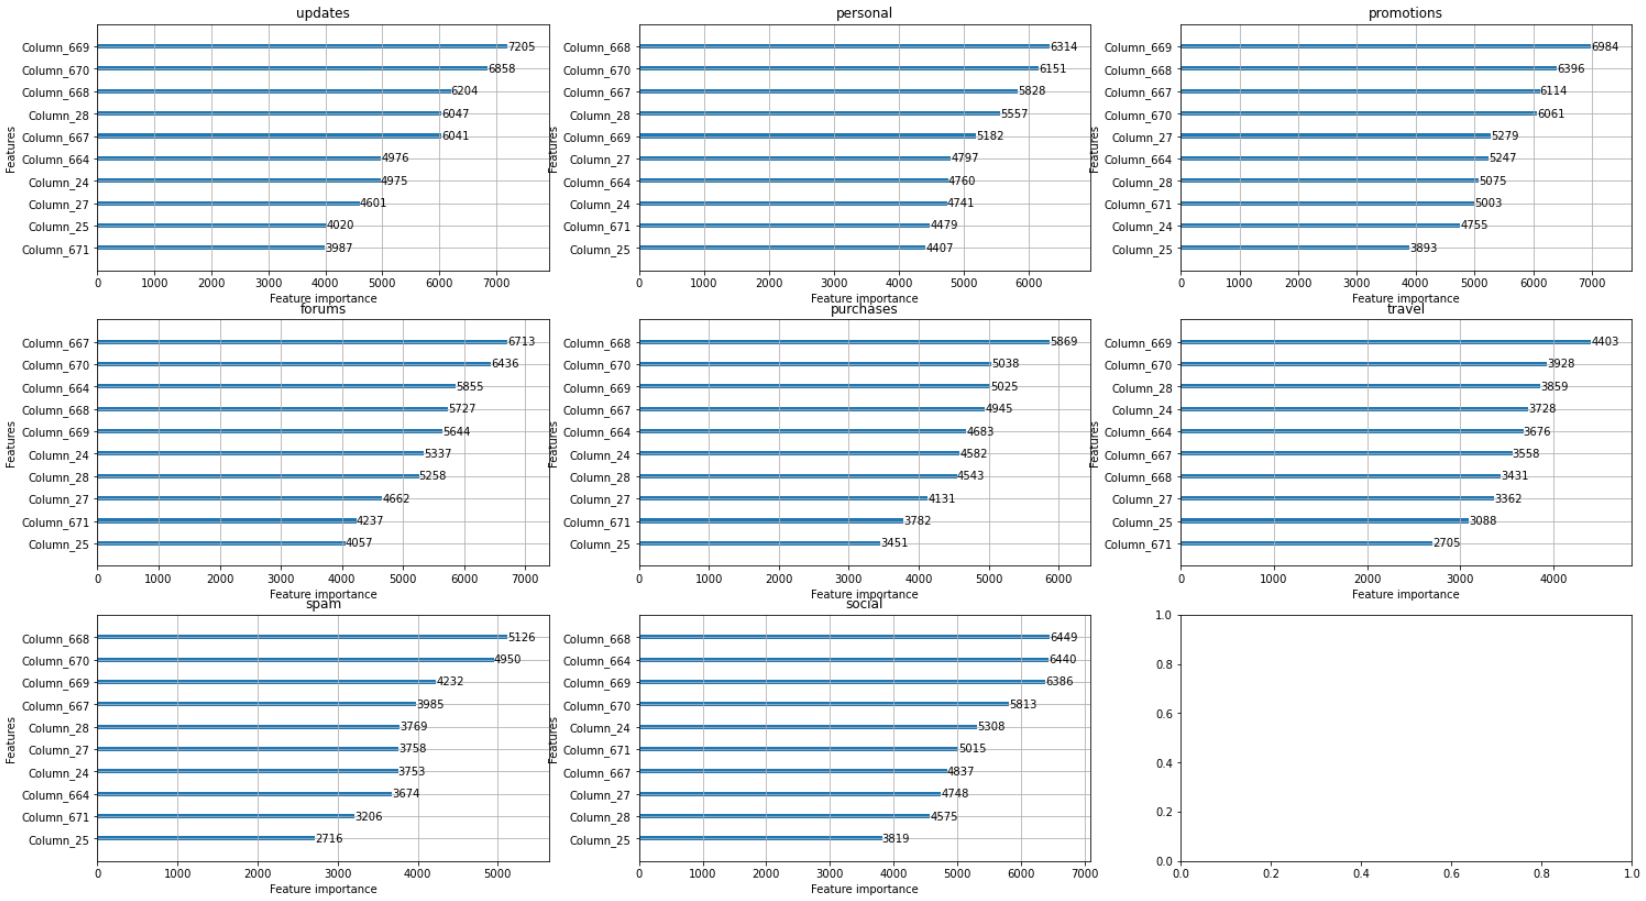
\includegraphics[scale=0.4]{Capture.PNG}
\caption{Feature importance for each class}
\label{fig:feature_importance}
\end{figure}

\begin{markdown}



The two most interesting features are `chars_in_subject/body` and `urls/body`. As a reminder, those custom features have been added because it wouldn't make sense to only consider `chars_in_subject` and `urls` as it is clear that a long mail have greater chance to have a high number of url links. In our case, it seems to be quite explanatory: we can easily think that `spam` and `promotions` have many links compared to its body while the others have a much lower ratio. The same goes for `chars_in_subject/body`: spams typically have a long subject field while personal mails tend to be much more concise.

However, it is quite surprising to see the feature importance of `minute`. Our guess is that all automated mails that are sent to a mailing list usually have their timestamp with an usual number for minutes ($0$, $15$,$30$ or $60$). On the contrary, `personal` and `social` probably have more uniformly distributed values.


\end{markdown}


\section{Model tuning and comparison}

In this part, we consider separately modern gradient boosting methods such as XGBoost or LightGBM.

\subsection{Classic machine learning techniques}
\begin{markdown}

To choose the models to use, we trained different models on the same dataset :

- DummyClassifier : Classifier that makes predictions using simple rules. Used to be a baseline.
- RandomForest : Classifier composed of many decisions trees and which uses bagging and feature randomness when building each of those individual tree to try to create an uncorrelated forest of trees whose prediction by committee is more accurate than that of any individual tree.
- Gradient Boosting : Classifier composed of many basic decision trees, trained in a sequential way, trying to minimize a certain cost function.
- Multi Layer Perceptron : Neural network model that optimizes the log-loss function using LBFGS or stochastic gradient descent.
- Linear models with stochastic gradient descent (SGD) : we use first a kernel approximation called _Nystroem_ to achieve better performances.

\end{markdown}

We obtain the following log-loss errors for each model without fine tuning :

\begin{table}[h!]
\begin{center}
 \begin{tabular}{|c | c | c | c | c|} 
 \hline
  DummyClassifier & RandomForest & Gradient Boosting & MLP & SGD \\ [0.5ex] 
  \hline
  2.27 & 1.19 & 1.38 & 1.66 & 1.63 \\
  \hline
\end{tabular}
\end{center}
\end{table}

In view of these results, we decide to focus only on random forest and to look for fine tuning.

First, we notice that the features to predict are really different in terms of frequency or complexity. We thus seek to evaluate the optimal number of estimators per class to be predicted, i.e. fine-tuning a random forest per class rather than using a OneVsRest type method.

Since the class are largely imbalanced, we have used cross-validation by stratifying with respect to y in order to have the same ratio of presence of classes in the train and test set. The results are given in Figures \ref{fig:down.png} and \ref{fig:up.png} which is the same plot but in two parts for readability purpose.

\begin{figure}[!tbp]
  \centering
  \begin{minipage}[bh!]{0.4\textwidth}
    \includegraphics[width=\textwidth]{data/down.png}
    \caption{Bottom part of the GridSearch for \text{n\_estimators}}
    \label{fig:down.png}
  \end{minipage}
  \hfill
  \begin{minipage}[bh!]{0.4\textwidth}
    \includegraphics[width=\textwidth]{data/up.png}
    \caption{Upper part of the GridSearch for \text{n\_estimators}}
    \label{fig:up.png}
  \end{minipage}
\end{figure}

In order to limit the complexity of the models and to avoid long training times or overfit, we use the following values:

\begin{table}[h!]
\begin{center}
 \begin{tabular}{|c | c | c | c | c | c | c | c|} 
 \hline
  updates & personal & promotions & forums & purchases & travel & spam & social\\ [0.5ex] 
  \hline
  400 & 400 & 300 & 200 & 300 & 400 & 200 & 200\\
  \hline
\end{tabular}
\end{center}
\caption{Optimal number of estimators for random forest per class}
\end{table}

We get a log-loss of about 0.06 on the Kaggle competition. To improve our score, we are turning to more advanced methods.

\subsection{Modern Gradient Boosting machine learning techniques}

Light GBM and XGBoost are advanced Gradient Boosting methods that support parallel training, multiple loss functions, regularization, bagging and early stopping.
One of the strong points of the model is that it manages itself the missing values, and the encoding.

We used the following filter on our predictions: 
$$\frac{\sin\left((x-0.5)*\pi\right)}{2}+0.5$$
\begin{markdown}
Indeed, we see that this function spreads the values of $x$ away from 0.5, which can be interpreted as "forcing" the algorithm to take a decision since we don't want an indecisive model. This has proved successful since the model improved of around 0.02.
\end{markdown}


We get a log-loss of about 0.05 on the Kaggle competition with a Light GBM. A good improvement over a Random Forest!

\end{document}